\question{Câu 14}

Cho 3 dạng sóng $V_{1}(t)$, $V_{2}(t)$ và $V_{3}(t)$ như hình vẽ. Thiết kế mạch biến đổi sử dụng OPAMP có 2 ngõ ra là $V_{1}(t)$ và $V_{2}(t)$, mạch cho ngõ ra là dạng sóng $V_{3}(t)$. Giả sử OPAMP sử dụng là lý tưởng.

\begin{figure}[H]
	\centering
	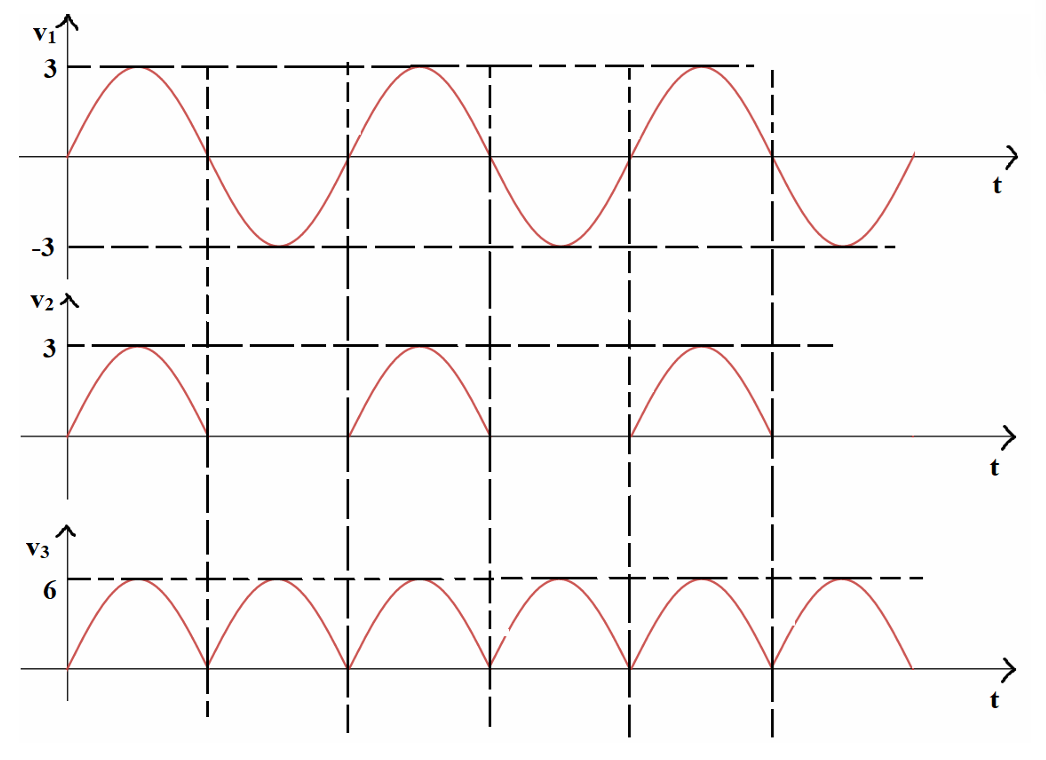
\includegraphics[width=\linewidth]{./my-chapters/my-images/Question14/debai.png}
	\caption*{Hình 14.}
\end{figure}

\answer{a}{Thiết kế mạch.}

Trước hết ta cần tạo tính hiệu $V_{2}$ từ tín hiệu hình sin nhưng chỉ lấy bán kỳ dương ta sử dụng cấu trúc mạch Active Clipper sử dụng opamp.

\begin{figure}[H]
	\centering
	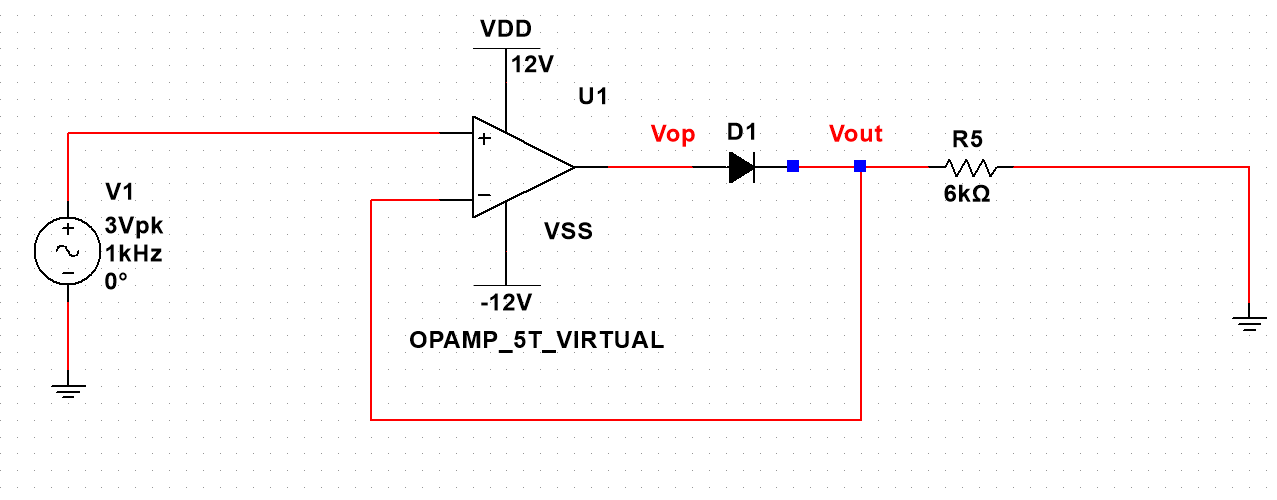
\includegraphics[width=.8\linewidth]{./my-chapters/my-images/Question14/C14_Hình1.png}
	\caption{Mạch Active Clipper.}
\end{figure}

Ở trang thái ban đầu $V_{-} = V_{out} = 0$, $V_{+} = V_{in}$

\begin{itemize}[label=-]
	\item Khi $V_{in} > 0 \rightarrow V_{op} = V_{OH} \rightarrow D_{1} \text{ dẫn } \Rightarrow$ Mạch đóng gói vai trò như buffer $\rightarrow V_{out} = V_{in}$.
	\item Khi $V_{in} < 0 \rightarrow V_{op} = V_{OL} \rightarrow D_{1} \text{ tắt } \Rightarrow$ $V_{out} = 0$.
\end{itemize}

\begin{figure}[H]
	\centering
	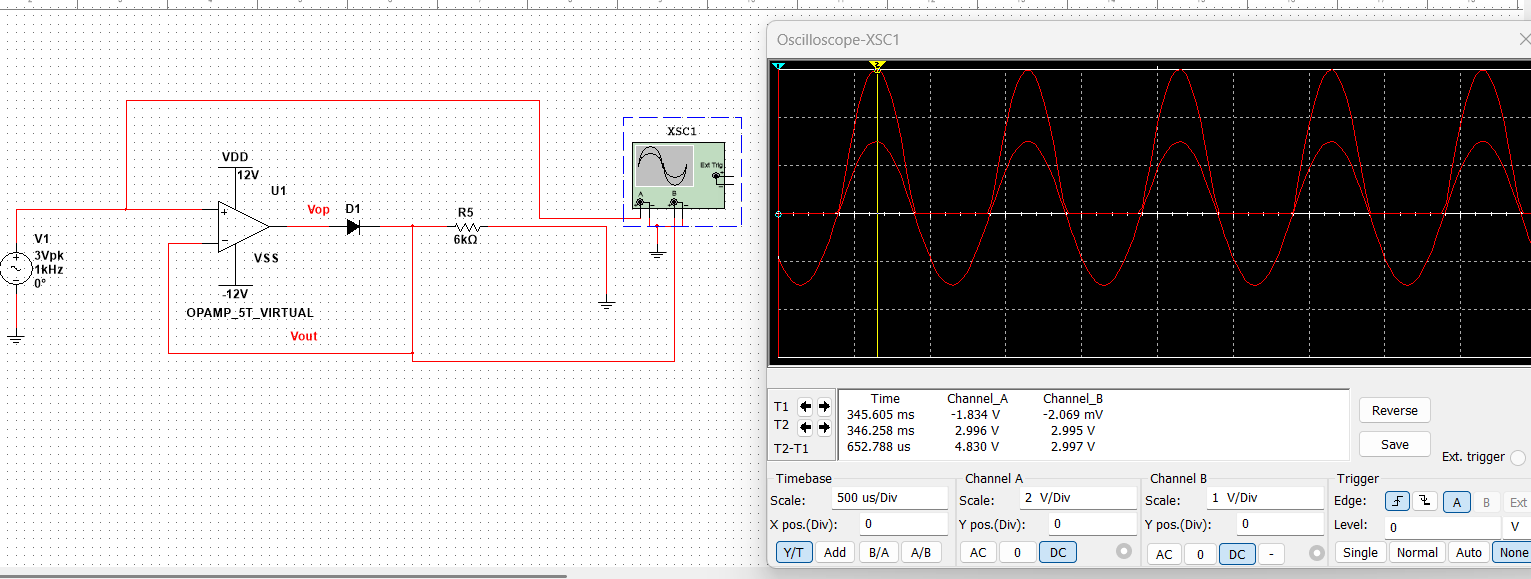
\includegraphics[width=.8\linewidth]{./my-chapters/my-images/Question14/C14_Hình2.png}
	\caption{Tạo điện áp $V_{2}$.}
\end{figure}

Từ đồ thị $V_{3} \rightarrow V_{3} = 4V_{2} - 2V_{1} $. Tạo điện áp $4V_{2}$ và $-2V_{1}$ từ Inverting Amplifier và Non Inverting Amplifier.

\begin{figure}[H]
	\centering
	\begin{minipage}{.48\linewidth}
		\centering
		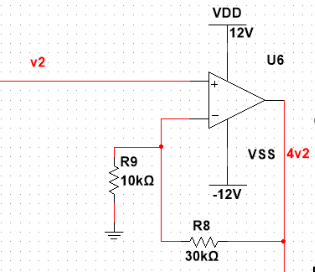
\includegraphics[width=.9\linewidth]{./my-chapters/my-images/Question14/C14_Hình3_1.png}
		\caption*{(a)}
	\end{minipage}%
	\hfill
	\begin{minipage}{.48\linewidth}
		\centering
		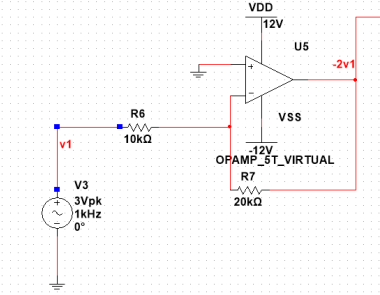
\includegraphics[width=.9\linewidth]{./my-chapters/my-images/Question14/C14_Hình3_2.png}
		\caption*{(b)}
	\end{minipage}
	\caption{Tạo điện áp $4V_{2}$ và $-2V_{1}$.}
\end{figure}

Tiếp đến sử dụng cấu trung Non Inverting Summing Amplifier để cộng 2 điện áp $4V_{2}$ và $-2V_{1}$ thành $V_{3}$

\begin{figure}[H]
	\centering
	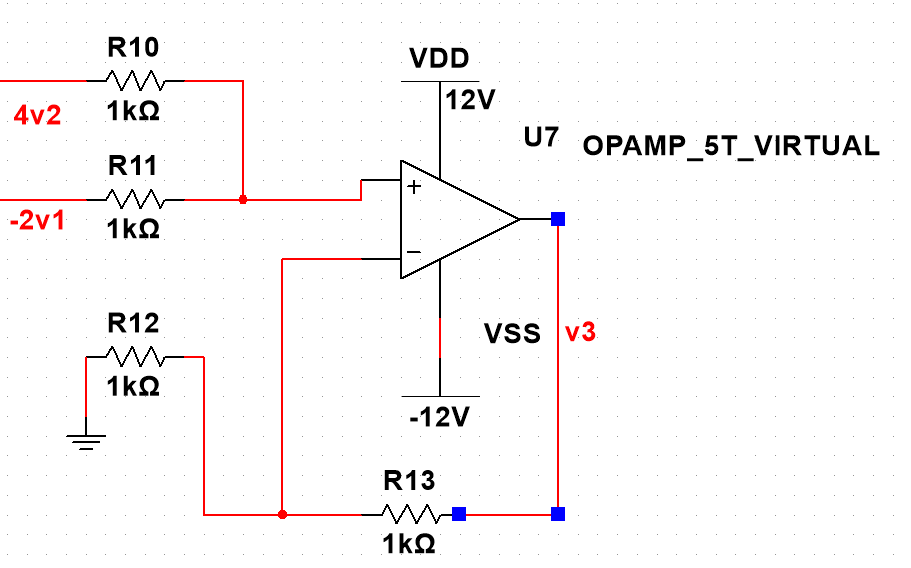
\includegraphics[width=.8\linewidth]{./my-chapters/my-images/Question14/C14_Hình4.png}
	\caption{Tạo điện áp $V_{3}$.}
\end{figure}

\answer{b}{Mô phỏng mạch dùng Multisim (hoặc các chương trình tương tự).}

\begin{figure}[H]
	\centering
	
\includegraphics[width=\linewidth]{./my-chapters/my-images/Question14/C14_Hình5.png}
	\caption{Mạch sau hoàn chỉnh.}
\end{figure}

\begin{figure}[H]
	\centering
	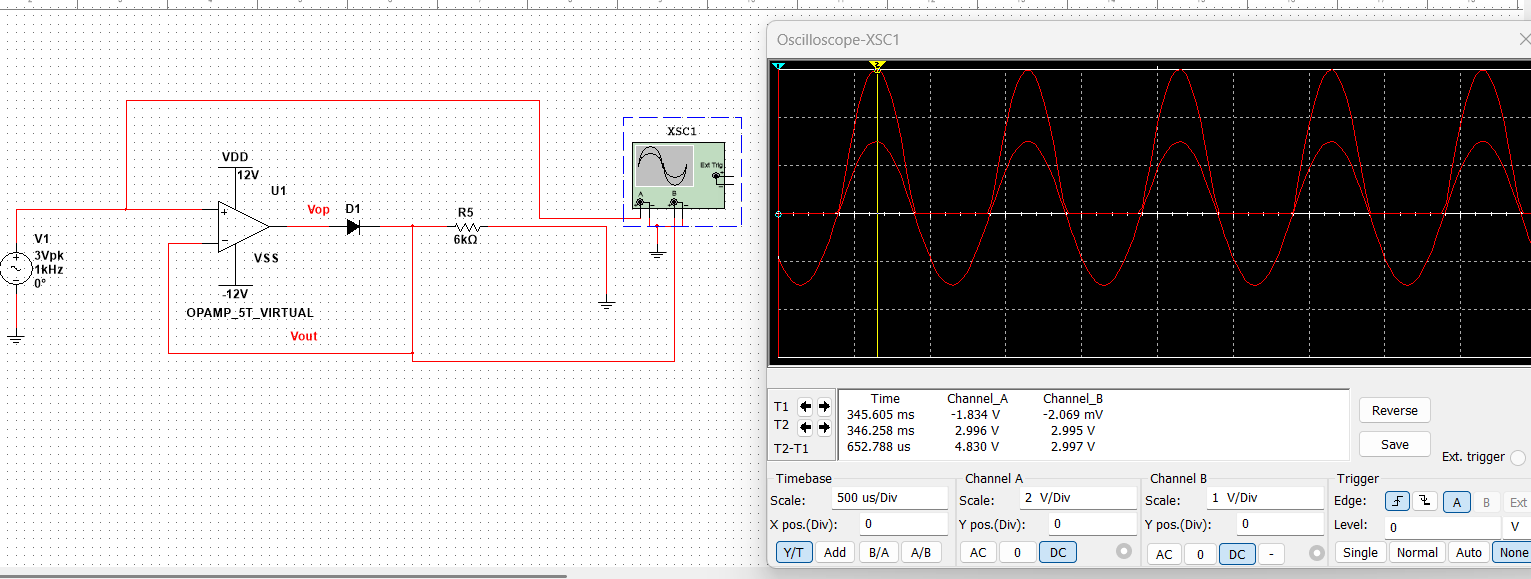
\includegraphics[width=\linewidth]{./my-chapters/my-images/Question14/C14_Hình2.png}
	\caption{Mô phỏng Multisim $V_{2}$.}
\end{figure}


\begin{figure}[H]
	\centering
	
\includegraphics[width=\linewidth]{./my-chapters/my-images/Question14/C14_Hình6.png}
	\caption{Mô phỏng Multisim $V_{3}$.}
\end{figure}

